\section{Attend, Infer, Repeat (\textsc{AIR})}
\label{sec:air}

% recap of AIR
\gls{AIR}, introduced by \cite{Eslami2016air}, is a structured \gls{VAE} capable of decomposing a static scene $\bx$ into its constituent objects, where each object is represented as a separate triplet of continuous latent variables $\bz = \{\bz^{\mathrm{what}, i}, \bz^{\mathrm{where}, i}, z^{\mathrm{pres},i}\}_{i=1}^n$, $n \in \mathbb{N}$ being the (random) number of objects in the scene.
Each triplet of latent variables explicitly encodes position, appearance and presence of the respective object, and the model is able to infer the number of objects present in the scene. Hence it is able to count, locate and describe objects in the scene, all learnt in an unsupervised manner, made possible by the inductive bias introduced by the model structure.

\textbf{Generative Model}
The generative model of \gls{AIR} is defined as follows
\begin{align}
\label{eq:air_gen}
    \p{n}{}{\theta} &= \mathrm{Geom} (n \mid \theta), 
    &
    \p{\bz^{\mathrm{w}}}{n}{\theta} &= \prod_{i=1}^n \p{\bz^{w,i}}{}{\theta} = \prod_{i=1}^n \gauss{\bz^{w,i}|\bf{0}, \bf{I}},\nonumber \\
    \p{\bx}{\bz}{\theta} &= \gauss{\bx \mid \byt, \sigma^2_x \bm{I}}, 
    &\text{with}~~\byt &= \sum_{i=1}^n \operatorname{h}^\mathrm{dec}_\theta (
        \bz^{\mathrm{what}, i}, \bz^{\mathrm{where}, i}
    ),
\end{align}
where $\bz^{\mathrm{w},i} \defeq (\bz^{\mathrm{what}, i}, \bz^{\mathrm{where}, i})$, $z^{\mathrm{pres}, i}=1$ for $i=1 \ldots n$ and $h^\mathrm{dec}_\theta$ is the object decoder with parameters $\theta$.
It is composed of a \textit{glimpse decoder} $f_\theta^\mathrm{dec}: \bgt^i \mapsto \byt^i$,
which constructs an image patch and a 
spatial transformer ($\operatorname{ST}$, \cite{Jaderberg2015}), which scales and shifts it according to $\bz^\mathrm{where}$; see \Cref{fig:generation} for details.

\textbf{Inference}
\cite{Eslami2016air} use a sequential inference algorithm, where latent variables are inferred one at a time; see \Cref{fig:sqair_inf_flow}.
The number of inference steps $n$ is given by $z^{\mathrm{pres}, 1:n+1}$, a random vector of $n$ ones followed by a zero. The $\bz^{i}$ are sampled sequentially from
\vspace{-7pt}
\begin{equation} \label{eq:air_posterior}
    \q{\bz}{\bx}{\phi} = 
        \q{z^{\mathrm{pres}, n+1} = 0}{\bz^{\mathrm{w}, 1:n}, \bx}{\phi} 
        \prod_{i=1}^n 
        \q{\bz^{\mathrm{w}, i}, z^{\mathrm{pres}, i} = 1}{\bz^{1:i-1}, \bx}{\phi},
\end{equation}
where $q_\phi$ is implemented as a neural network with parameters $\phi$. 
To implement explaining away, e.g.\ to avoid encoding the same object twice, it is vital to capture the dependency of $\bz^{\mathrm{w},i}$ and  $z^{\mathrm{pres}, i}$ on $\bz^{1:i-1}$ and $\bx$. This is done using a \gls{RNN} $R_\phi$ with hidden state $\bm{h}^i$, namely:
$
    \bm{\omega}^i, \bm{h}^i = R_\phi (\bx, \bz^{i-1}, \bm{h}^{i-1}).
$
The outputs $\bm{\omega}^i$, which are computed iteratively and depend on the previous latent variables (\textit{cf}. \Cref{algo:sqair_disc}), parametrise $\q{\bz^{\mathrm{w},i}, \bz^{\mathrm{pres},i}}{\bz^{1:i-1}, \bx}{\phi}$. For simplicity the latter is assumed to factorise such that
$
    \q{\bz^{\mathrm{w}}, \bz^{\mathrm{pres}}}{\bz^{1:i-1}, \bx}{\phi} = \q{z^{\mathrm{pres}, n+1} = 0}{\bm{\omega}^{n+1}}{\phi} \prod_{i=1}^n \q{\bz^{\mathrm{w},i}}{\bm{\omega}^i}{\phi} \q{z^{\mathrm{pres}, i} = 1}{\bm{\omega}^i}{\phi}.
$

\begin{figure}
    \centering
    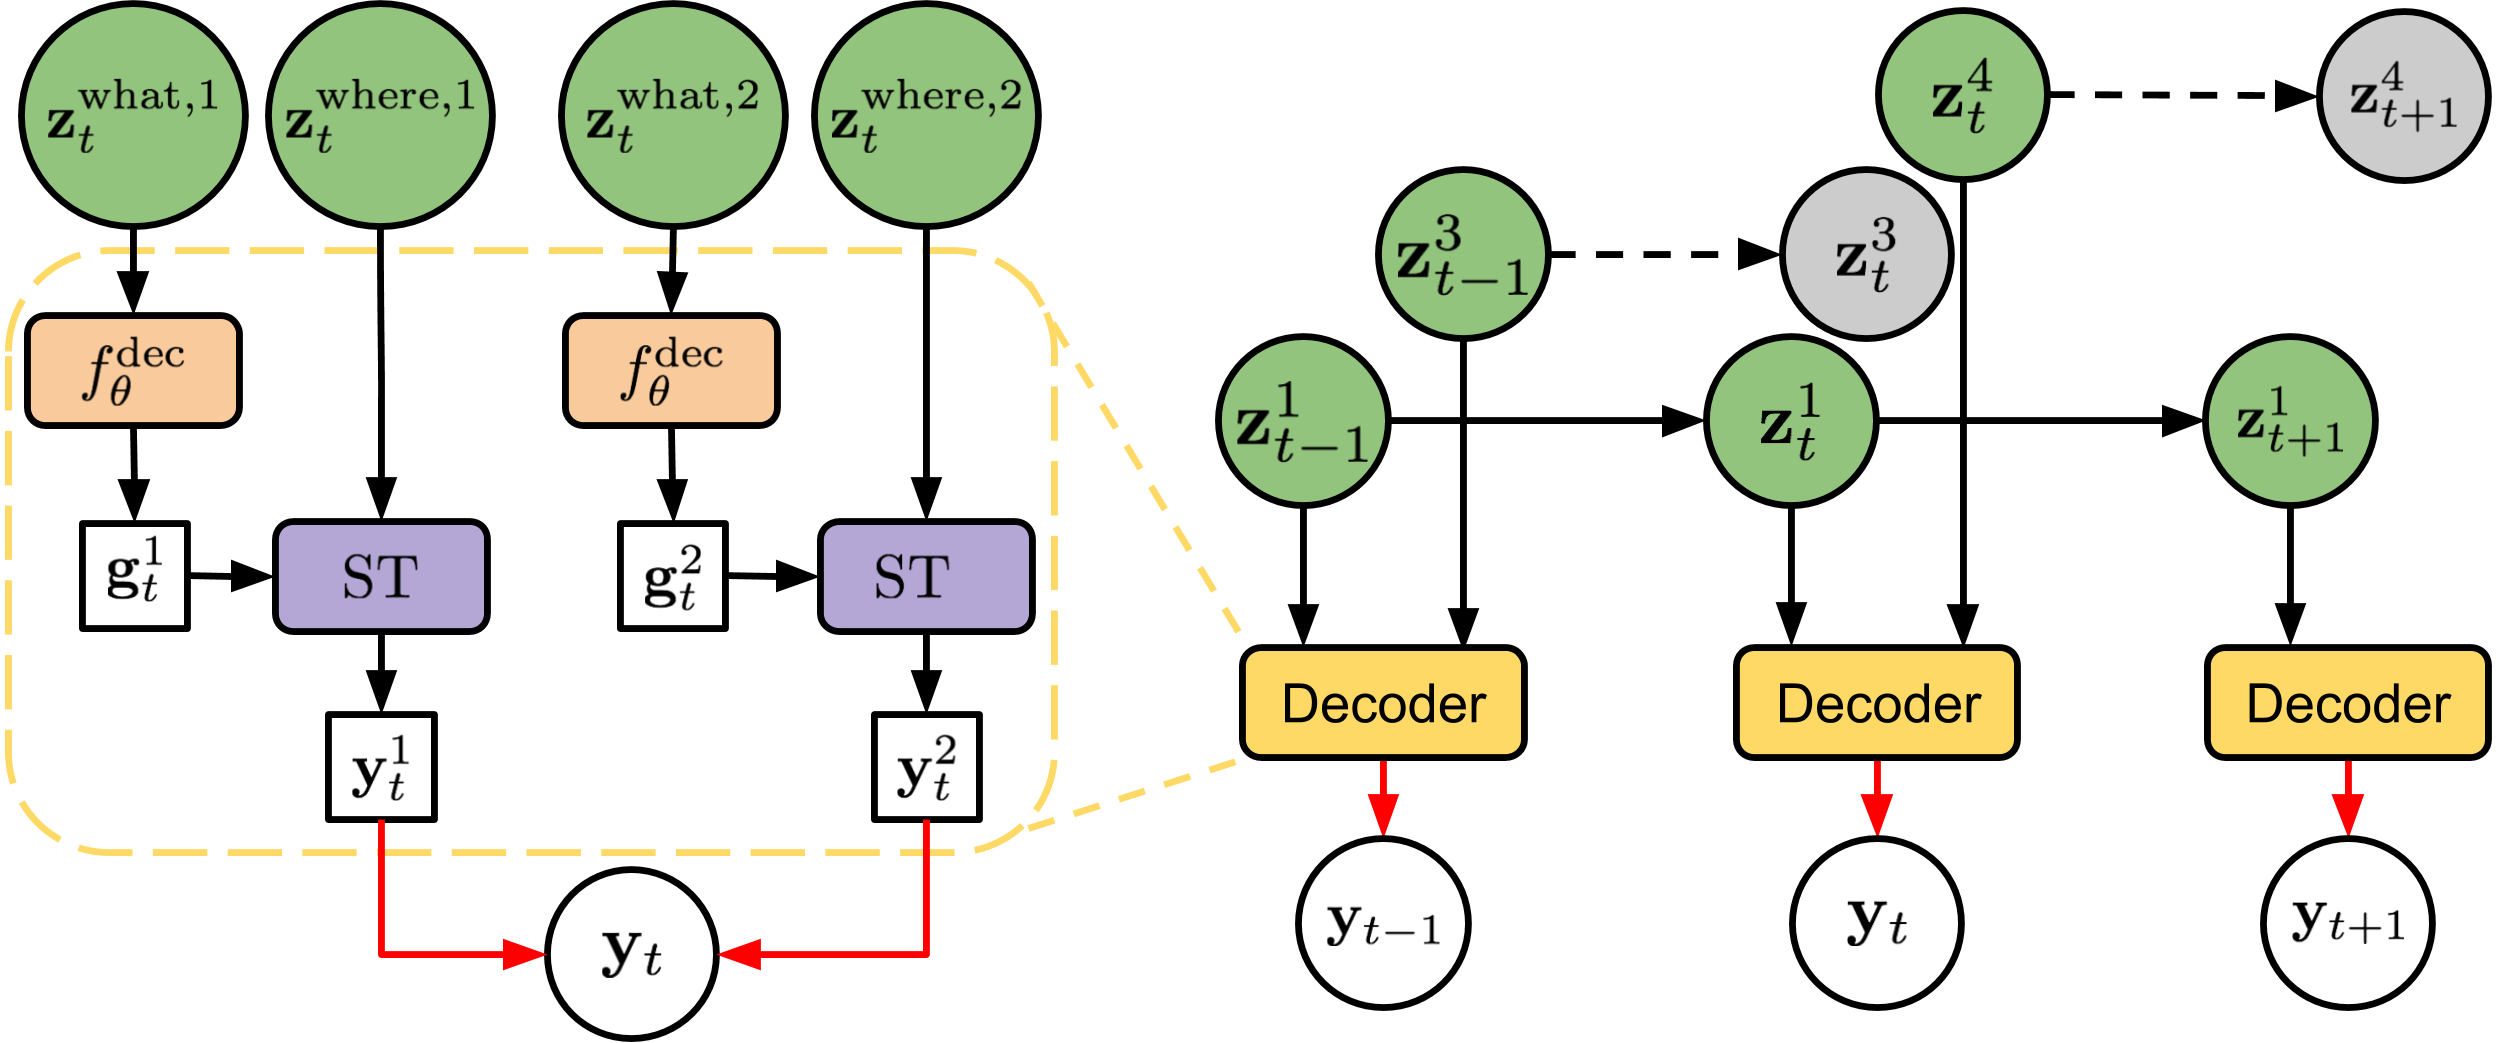
\includegraphics[width=0.7\linewidth]{figures/SQAIR/air_sqair_generation}
    \caption{
        \textit{Left}:
            Generation in \gls{AIR}.
            The image mean $\byt$ is generated by first using the \textit{glimpse decoder} $f_\theta^\mathrm{dec}$ to map the \textit{what} variables into glimpses $\bgt$, transforming them with the \textit{spatial transformer} $\STN$ according to the \textit{where} variables and summing up the results.
        \textit{Right}:
            Generation in \gls{SQAIR}.
%            When new objects enter the frame, new latent variables (here, $\bzt^4$) are sampled from the \textit{discovery} prior. The temporal evolution of already present objects is governed by the \textit{propagation} prior, which can choose to forget some variables (here, $\bzt^3$ and $\bz_{t+1}^4$) when the object moves out of the frame. The image generation process, which mimics the left-hand side of the figure, is abstracted in the \textit{decoder} block. 
    }
    \label{fig:generation}
\end{figure}

